


%	PACKAGES AND OTHER DOCUMENT CONFIGURATIONS

\documentclass[
	12pt, % Default font size, values between 10pt-12pt are allowed
	%letterpaper, % Uncomment for US letter paper size
	%spanish, % Uncomment for Spanish
]{style/fphw}

% Template-specific packages

\usepackage[utf8]{inputenc} % Required for inputting international characters
\usepackage[T1]{fontenc} % Output font encoding for international characters
\usepackage{mathpazo} % Use the Palatino font
\usepackage{amssymb}
\usepackage{graphicx} % Required for including images
\usepackage{booktabs} % Required for better horizontal rules in tables
\usepackage{listings} % Required for insertion of code
\usepackage{enumerate} % To modify the enumerate environment
\usepackage{epstopdf}
% \epstopdfDeclareGraphicsRule{.tif}{png}{.png}{convert #1 \OutputFile}
\AppendGraphicsExtensions{.tif}
\usepackage[ruled,vlined]{algorithm2e}
\usepackage{minted}
\usepackage[nottoc]{tocbibind}
\usepackage{caption}
\usepackage{subcaption}
\usepackage{mathtools}
\DeclarePairedDelimiter\abs{\lvert}{\rvert}%
\DeclarePairedDelimiter\norm{\lVert}{\rVert}%

% Swap the definition of \abs* and \norm*, so that \abs
% and \norm resizes the size of the brackets, and the 
% starred version does not.
\makeatletter
\let\oldabs\abs
\def\abs{\@ifstar{\oldabs}{\oldabs*}}
%
\let\oldnorm\norm
\def\norm{\@ifstar{\oldnorm}{\oldnorm*}}
\makeatother



\graphicspath{{/Users/tongyuan/Documents/Study/S6_Spring_2021/Digital_Imagine_Processing/EE326_Digital_Image_Processing_LAB/Lab6_Image_Restoration/plots}}

%----------------------------------------------------------------------------------------
%	ASSIGNMENT INFORMATION
%----------------------------------------------------------------------------------------

\title{Lab 6 Frquency Domain Filtering} % Assignment title

\author{YUAN Tong 11810818} % Student name

%\date{March 28th, 2025} % Due date

\institute{Southern University of Science and Technology \\ School of Microelectronic} % Institute or school name

\class{LAB Session I} % Course or class name

\professor{YU Yajun} % Professor or teacher in charge of the assignment

%----------------------------------------------------------------------------------------

\begin{document}
\definecolor{bg}{rgb}{0.95,0.95,0.95}
\maketitle % Output the assignment title, created automatically using the information in the custom commands above

%----------------------------------------------------------------------------------------
%	ASSIGNMENT CONTENT
%----------------------------------------------------------------------------------------

\section*{Introduction}
The objective of restoration is to improve a given image in some predefined sense. Compare with image enhancement which is largely a subjective process, image restoration is for the most part an objective process. When we apply image restoring to a degraded image, we will first construct a model about how the image was degraded and then we apply the degrade filter to the restoring filter. After that we could get the reconstructed image, however, we can't build the degrade model precisely and there may be some overlap in frequency domain after the image was degrade, so we can not always restore that image like what it used to be.

In this lab, there are three tasks will be performed.

\begin{enumerate}
	\item Apply adeptive filter to the image with high noise intensity
	\item Apply full inverse filtering, radially limited inverse filtering and Wiener filtering to a image degraded by atomsphere turbulence. Discuss how the parameters, if any, are determined, and the different effects by using the different algorithms.
	\item Restore a image degraded by motion blur and noise.
\end{enumerate}

%----------------------------------------------------------------------------------------
%	TASKS
%----------------------------------------------------------------------------------------

\newpage
\section*{Task I: Adaptive Filter for Image Denoising}

\begin{problem}
	Remove the noise from the input images Q6\_1\_1.tif, Q6\_1\_2.tif, Q6\_1\_3.tif and Q6\_1\_4.tif. Explain your observation and the method used to each of the images, and why such methods are used.

	\begin{figure}[H]
		\centering
		\begin{subfigure}[b]{.2\textwidth}
			\centering
			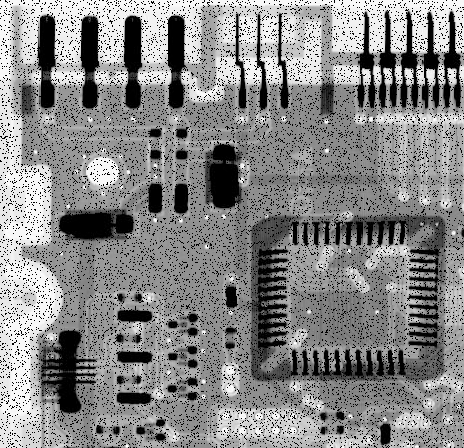
\includegraphics[width=0.9\linewidth]{Q6_1_1.png}
			\caption{Q6\_1\_1}
			\label{Q6_1_1}
		\end{subfigure}
		\hfill
		\begin{subfigure}[b]{.2\textwidth}
			\centering
			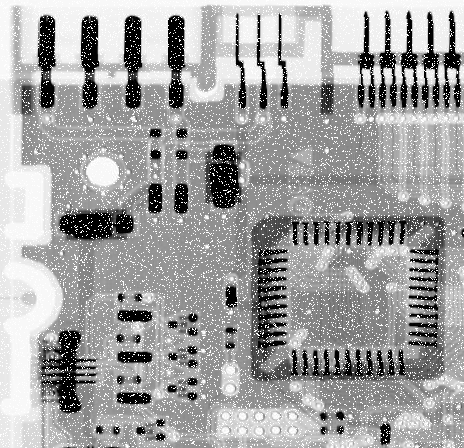
\includegraphics[width=0.9\linewidth]{Q6_1_2.png}
			\caption{Q6\_1\_2}
			\label{Q6_1_2}
		\end{subfigure}
		\hfill
		\begin{subfigure}[b]{.2\textwidth}
			\centering
			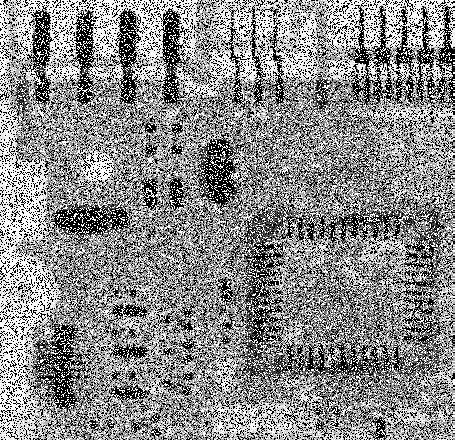
\includegraphics[width=0.9\linewidth]{Q6_1_3.png}
			\caption{Q6\_1\_3}
			\label{Q6_1_3}
		\end{subfigure}
		\hfill
		\begin{subfigure}[b]{.2\textwidth}
			\centering
			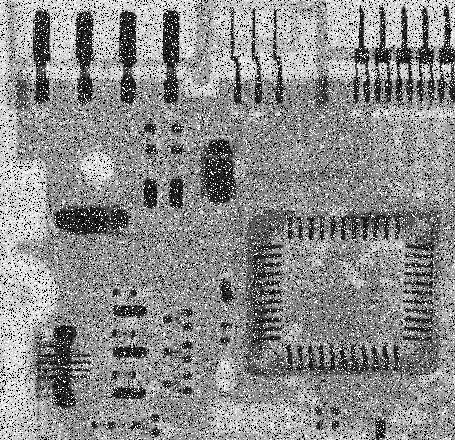
\includegraphics[width=0.9\linewidth]{Q6_1_4.png}
			\caption{Q6\_1\_4}
			\label{Q6_1_4}
		\end{subfigure}
		\caption{Task I, Figures with noise}
    	\label{Task I, Figures with noise}	
	\end{figure}
\end{problem}

\subsection*{Analysis}




\section*{Task II: Image Restoration}

\begin{problem}
	Image Q6\_2.tif was degraded from an original image due to the atmosphere turbulence given on slide 65 with k = 0.0025. Restore the original image from the input Q6\_2.tif by using full inverse filtering, radially limited inverse filtering and Wiener filtering. Discuss how the parameters, if any, are determined, and the different effects by using the different algorithms.

	\begin{figure}[H]
		\centering
	    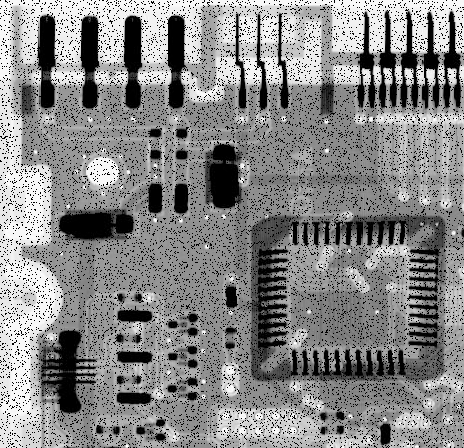
\includegraphics[width=0.3\linewidth]{Q6_1_1.png}
	    \caption{Q6\_1\_1}
	    \label{Q6_1_1}
	\end{figure}
\end{problem}


	

\section*{Task III: Motion Debluring}

\begin{problem}
	Restore the original images from the inputs Q6\_3\_1.tif, Q6\_3\_2.tif and Q6\_3\_3. Explain your observation and the method used.

	\begin{figure}[H]
		\centering
		\begin{subfigure}[b]{.3\textwidth}
			\centering
			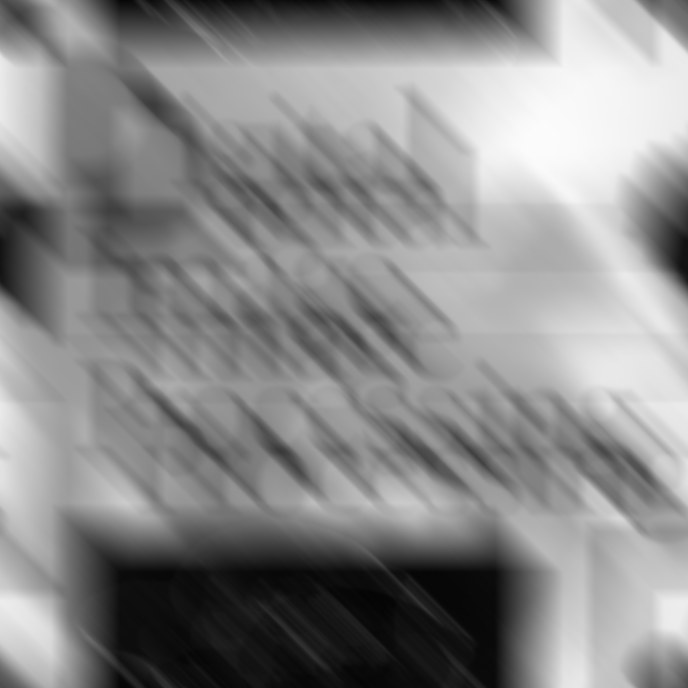
\includegraphics[width=0.9\linewidth]{Q6_3_1.png}
			\caption{Q6\_3\_1}
			\label{Q6_3_1}
		\end{subfigure}
		\hfill
		\begin{subfigure}[b]{.3\textwidth}
			\centering
			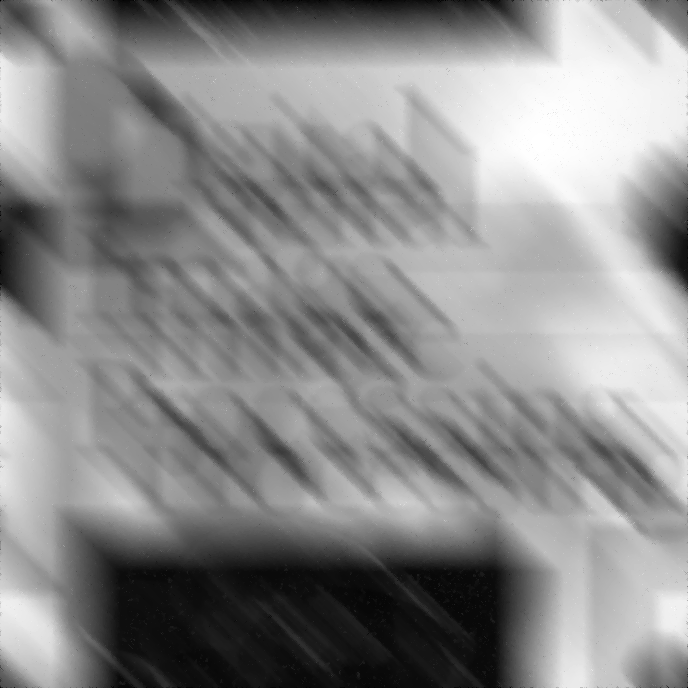
\includegraphics[width=0.9\linewidth]{Q6_3_2.png}
			\caption{Q6\_3\_2}
			\label{Q6_3_2}
		\end{subfigure}
		\hfill
		\begin{subfigure}[b]{.3\textwidth}
			\centering
			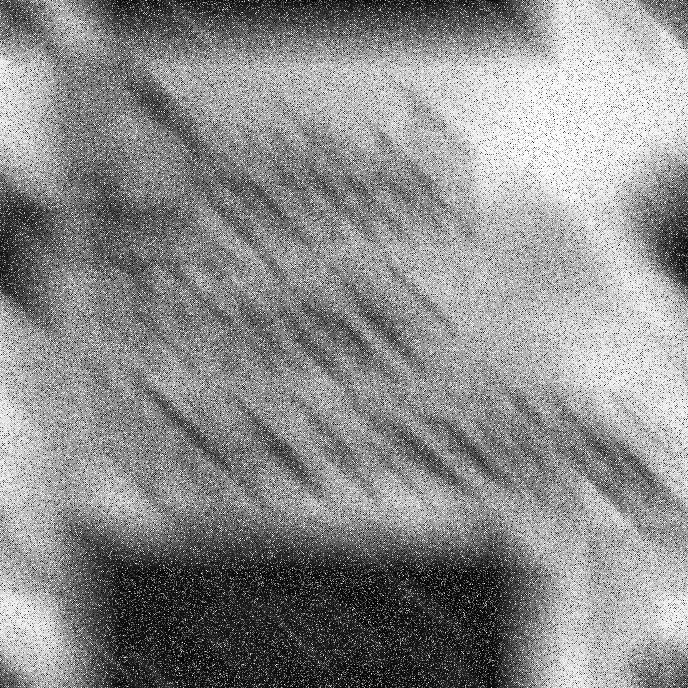
\includegraphics[width=0.9\linewidth]{Q6_3_3.png}
			\caption{Q6\_3\_3}
			\label{Q6_3_3}
		\end{subfigure}
		\caption{Task III, Figures with motion blur}
    	\label{Task III, Figures with motion blur}	
	\end{figure}

\end{problem}


\section*{Conclusion}



\end{document}
